\documentclass{oblivoir}
%%%Default packages
\usepackage{amsmath,amssymb,amsthm,kotex,tabu,graphicx,pifont}
\usepackage{../kswrapfig}

\usepackage{gensymb} %\degree

%%%More packages
%\usepackage{caption,subcaption}
%\usepackage[perpage]{footmisc}
%
\usepackage[skipabove=10pt,innertopmargin=10pt,nobreak=true]{mdframed}

\usepackage[inline]{enumitem}
\setlist[enumerate,1]{label=(\arabic*)}
\setlist[enumerate,2]{label=(\alph*)}

\usepackage{multicol}
\setlength{\columnsep}{30pt}
\setlength{\columnseprule}{1pt}
%
%\usepackage{forest}
%\usetikzlibrary{shapes.geometric,arrows.meta,calc}
%
%%%defi theo exam prob rema proo
%이 환경들 아래에 문단을 쓸 경우 살짝 들여쓰기가 되므로 \hspace{-.7em}가 필요할 수 있다.

\newcounter{num}
\newcommand{\defi}[1]
{\noindent\refstepcounter{num}\textbf{정의 \arabic{num})} #1\par\noindent}
\newcommand{\theo}[1]
{\noindent\refstepcounter{num}\textbf{정리 \arabic{num})} #1\par\noindent}
\newcommand{\revi}[1]
{\noindent\refstepcounter{num}\textbf{복습 \arabic{num})} #1\par\noindent}
\newcommand{\exam}[1]
{\bigskip\bigskip\noindent\refstepcounter{num}\textbf{예시 \arabic{num})} #1\par\noindent}
\newcommand{\prob}[1]
{\bigskip\bigskip\noindent\refstepcounter{num}\textbf{문제 \arabic{num})} #1\par\noindent}
\newcommand{\rema}[1]
{\bigskip\bigskip\noindent\refstepcounter{num}\textbf{참고 \arabic{num})} #1\par\noindent}
\newcommand{\proo}
{\bigskip\noindent\textsf{증명)}}

\newenvironment{talign}
 {\let\displaystyle\textstyle\align}
 {\endalign}
\newenvironment{talign*}
 {\let\displaystyle\textstyle\csname align*\endcsname}
 {\endalign}
%
%%%Commands

\newcommand{\procedure}[1]{\begin{mdframed}\vspace{#1\textheight}\end{mdframed}}

\newcommand\an[1]{\par\bigskip\noindent\textbf{문제 \ref{#1})}\par\noindent}

\newcommand\ann[2]{\par\bigskip\noindent\textbf{문제 \ref{#1})}\:\:#2\par\medskip\noindent}

\newcommand\ans[1]{\begin{flushright}\textbf{답 : }#1\end{flushright}}

\newcommand\anssec[1]{\bigskip\bigskip\noindent{\large\bfseries#1}}

\newcommand{\pb}[1]%\Phantom + fBox
{\fbox{\phantom{\ensuremath{#1}}}}

\newcommand\ba{\,|\,}

\newcommand\ovv[1]{\ensuremath{\overline{#1}}}
\newcommand\ov[2]{\ensuremath{\overline{#1#2}}}
%
%%%% Settings
%\let\oldsection\section
%
%\renewcommand\section{\clearpage\oldsection}
%
%\let\emph\textsf
%
%\renewcommand{\arraystretch}{1.5}
%
%%%% Footnotes
%\makeatletter
%\def\@fnsymbol#1{\ensuremath{\ifcase#1\or
%*\or **\or ***\or
%\star\or\star\star\or\star\star\star\or
%\dagger\or\dagger\dagger\or\dagger\dagger\dagger
%\else\@ctrerr\fi}}
%
%\renewcommand{\thefootnote}{\fnsymbol{footnote}}
%\makeatother
%
%\makeatletter
%\AtBeginEnvironment{mdframed}{%
%\def\@fnsymbol#1{\ensuremath{\ifcase#1\or
%*\or **\or ***\or
%\star\or\star\star\or\star\star\star\or
%\dagger\or\dagger\dagger\or\dagger\dagger\dagger
%\else\@ctrerr\fi}}%
%}   
%\renewcommand\thempfootnote{\fnsymbol{mpfootnote}}
%\makeatother
%
%%% 객관식 선지
\newcommand\one{\ding{172}}
\newcommand\two{\ding{173}}
\newcommand\three{\ding{174}}
\newcommand\four{\ding{175}}
\newcommand\five{\ding{176}}
\usepackage{tabto,pifont}
%\TabPositions{0.2\textwidth,0.4\textwidth,0.6\textwidth,0.8\textwidth}

\newcommand\taba[5]{\par\noindent
\one\:{#1}
\tabto{0.2\textwidth}\two\:\:{#2}
\tabto{0.4\textwidth}\three\:\:{#3}
\tabto{0.6\textwidth}\four\:\:{#4}
\tabto{0.8\textwidth}\five\:\:{#5}}

\newcommand\tabb[5]{\par\noindent
\one\:{#1}
\tabto{0.33\textwidth}\two\:\:{#2}
\tabto{0.67\textwidth}\three\:\:{#3}\medskip\par\noindent
\four\:\:{#4}
\tabto{0.33\textwidth}\five\:\:{#5}}

\newcommand\tabc[5]{\par\noindent
\one\:{#1}
\tabto{0.5\textwidth}\two\:\:{#2}\medskip\par\noindent
\three\:\:{#3}
\tabto{0.5\textwidth}\four\:\:{#4}\medskip\par\noindent
\five\:\:{#5}}

\newcommand\tabd[5]{\par\noindent
\one\:{#1}\medskip\par\noindent
\two\:\:{#2}\medskip\par\noindent
\three\:\:{#3}\medskip\par\noindent
\four\:\:{#4}\medskip\par\noindent
\five\:\:{#5}}
%
%%%% fonts
%
%\usepackage{fontspec, xunicode, xltxtra}
%\setmainfont[]{은 바탕}
%\setsansfont[]{은 돋움}
%\setmonofont[]{은 바탕}
%\XeTeXlinebreaklocale "ko"
\setlength{\tabulinesep}{3pt}
%%%%
\begin{document}

\title{수학(하) : 06 원의 방정식}
\author{}
\date{\today}
\maketitle
\tableofcontents
\newpage

%%trace
\section{자취문제}
\begin{center}
\fbox{\(\cdots\)를 만족시키는 점 \(P\)의 자취를 구하여라.}\\[10pt]
\fbox{\(\cdots\)를 만족시키는 점 \(P\)의 자취의 방정식을 구하여라.}\\[10pt]
\fbox{\(\cdots\)를 만족시키는 점 \(P\)가 그리는 도형의 방정식을 구하여라.}\\[10pt]
\fbox{\(\cdots\)를 만족시키는 점 \(P\)가 그리는 궤적을 구하여라.}
\end{center}
와 같은 수학문제가 있다.
이것을 `자취문제'라고 하자.

%
\exam{}\label{trace1}
예를 들어,
\vspace{-15pt}
\begin{center}
\fbox{두 점 \(A(1,0)\), \(B(5,0)\)에 대해 \(\ov PA=\ov PB\)을 만족시키는 점 \(P\)의 자취를 구하여라.}
\end{center}
라는 문제가 있다고 하자.

%\begin{center}
%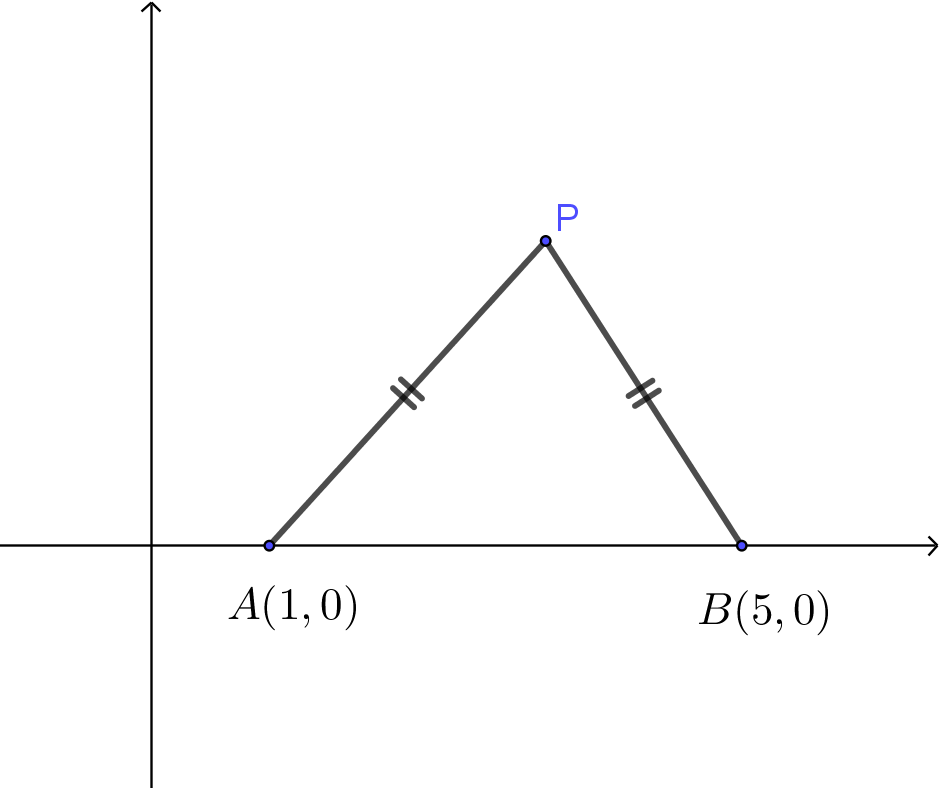
\includegraphics[width=.5\textwidth]{trace_1}
%\end{center}

\bigskip
\(P\)가 어떤 점일 때 \(\ov PA=\ov PB\)가 성립할까?
만약 \(P=(2,1)\)이거나 \(P=(5,2)\)이면 \(\ov PA\neq\ov PB\)이 되어 주어진 조건이 성립하지 않는다.
\begin{center}
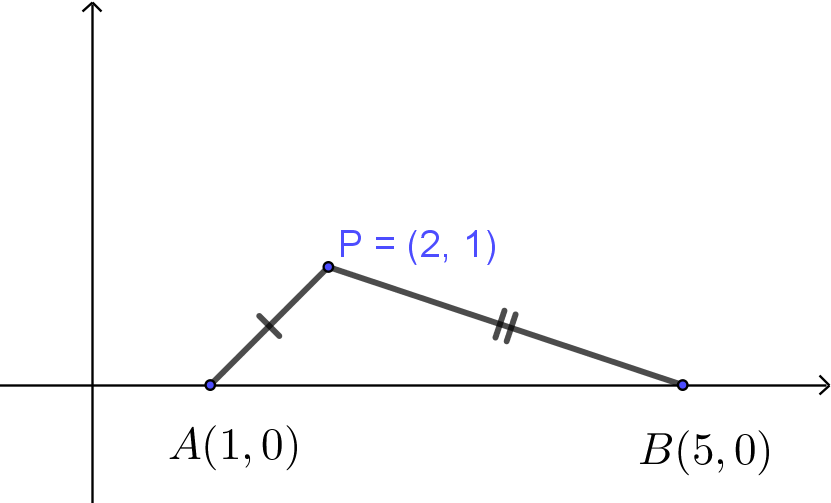
\includegraphics[width=.35\textwidth]{trace_1a}
~~
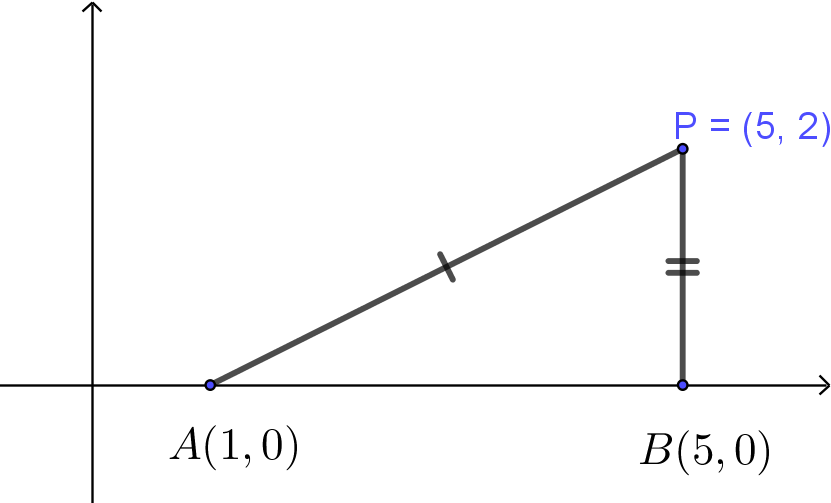
\includegraphics[width=.35\textwidth]{trace_1b}
\end{center}
하지만 \(P=(3,2)\)이거나 \(P=(3,1)\) 같은 점이면 주어진 조건 \(\ov PA=\ov PB\)가 성립한다.
\begin{center}
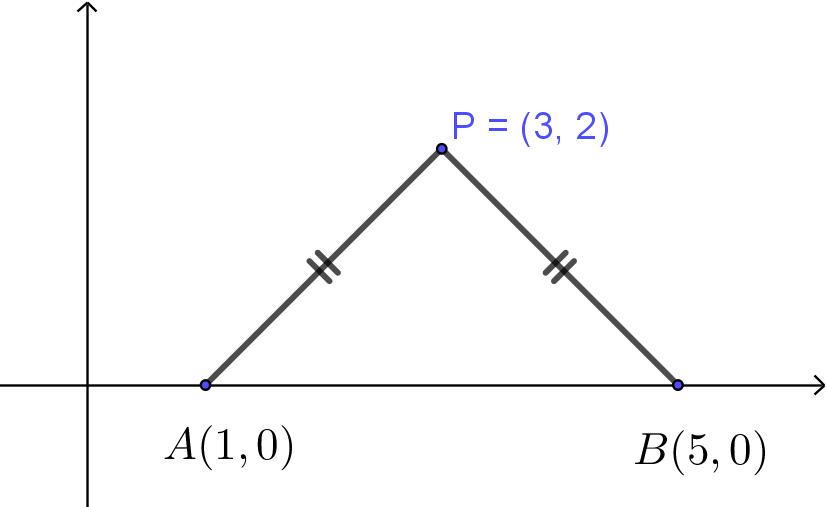
\includegraphics[width=.35\textwidth]{trace_1c}
~~
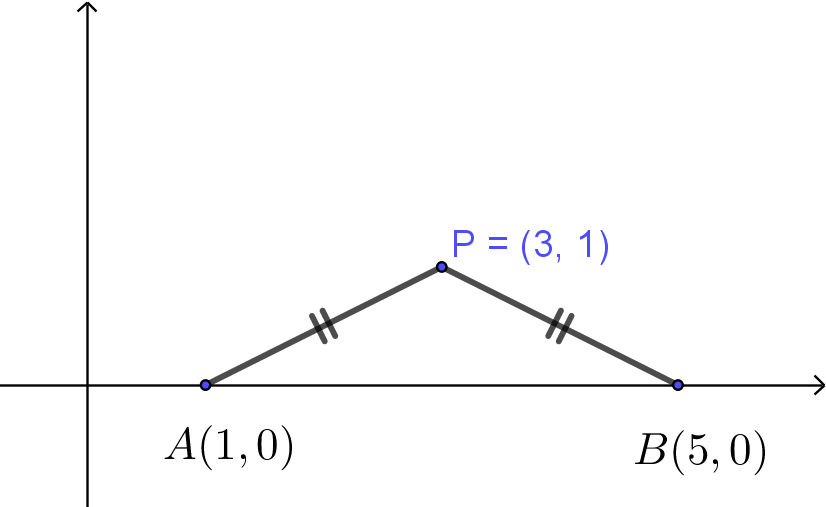
\includegraphics[width=.35\textwidth]{trace_1d}
\end{center}
조금만 더 생각해보면 점 \(P\)가 선분 \(AB\)의 수직이등분선인 \(x=3\) 위에 있으면 된다는 것을 알 수 있다.

\newpage
\noindent이 문제는 다음 두 방법으로 설명할 수 있다.
\begin{mdframed}[frametitle=풀이1]
점 \(P\)가 선분 \(AB\)의 수직이등분선 \(l\) 위에 있으면 주어진 조건 \(\ov PA=\ov PB\)가 성립한다.
하지만 점 \(P\)가 직선 \(l\)보다 왼쪽에 있으면 \(\ov PA<\ov PB\)이고 오른쪽에 있으면 \(\ov PA>\ov PB\)이다.
즉 \(P\)가 \(l\) 위에 있지 않으면 주어진 조건 \(\ov PA=\ov PB\)가 성립하지 않는다.
\begin{center}
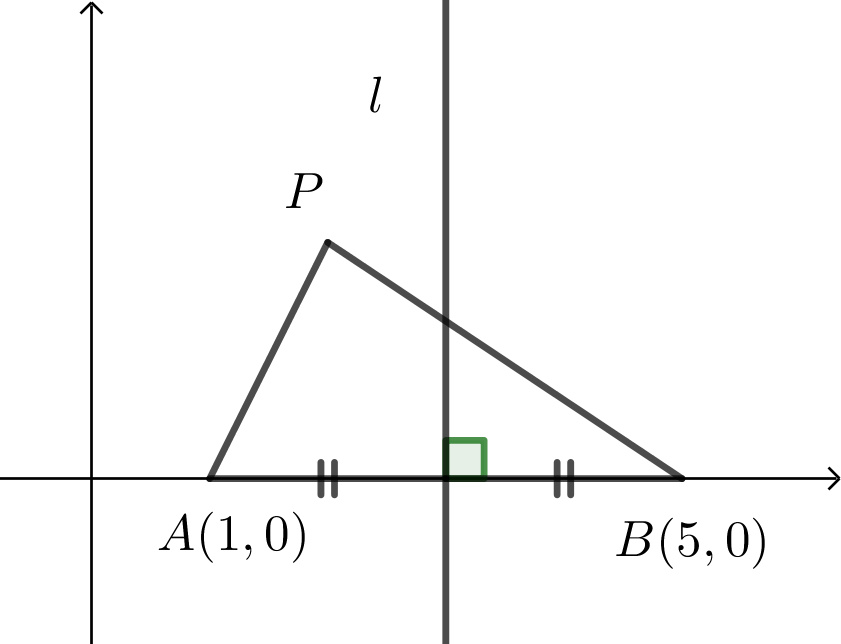
\includegraphics[width=0.25\textwidth]{trace_1-1}\qquad
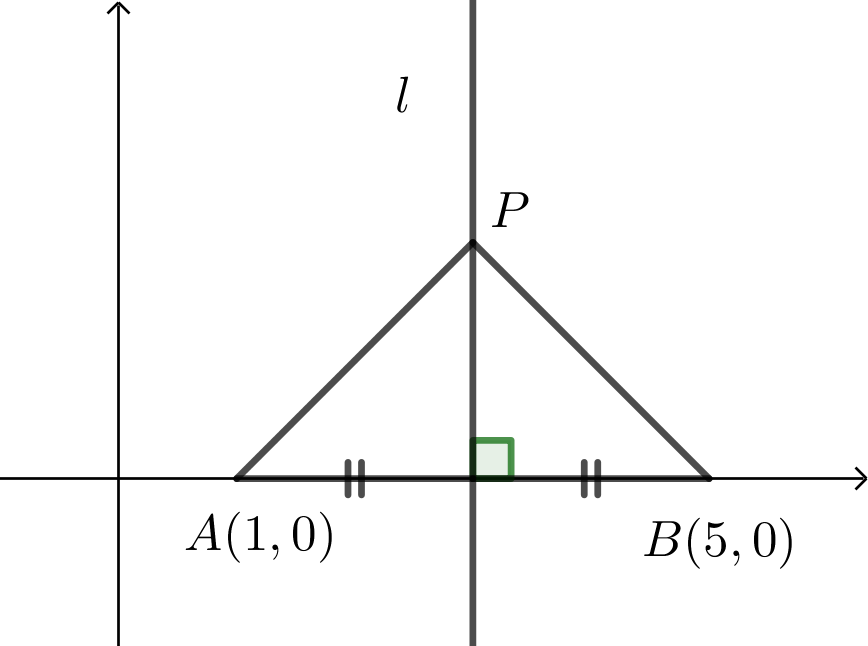
\includegraphics[width=0.25\textwidth]{trace_1-2}\qquad
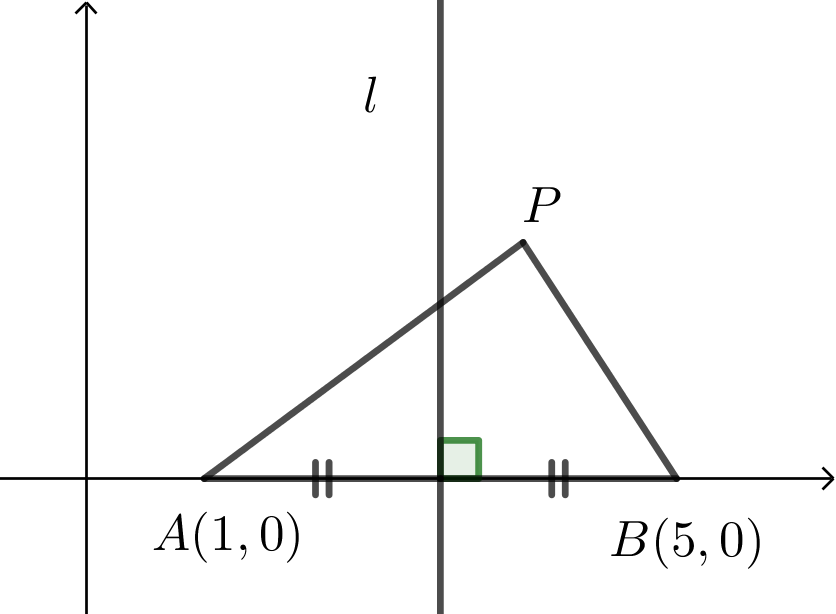
\includegraphics[width=0.25\textwidth]{trace_1-3}\\
\(\ov PA<\ov PB\)\qquad\qquad\qquad
\(\ov PA=\ov PB\)\qquad\qquad\qquad
\(\ov PA>\ov PB\)
\end{center}
따라서 \(P\)의 자취는 선분 \(AB\)의 수직이등분선이다.
\end{mdframed}

\begin{mdframed}[frametitle=풀이2]
구하는 점 \(P\)를
\[P=(x,y)\]
라고 두자.
그러면 \(\ov PA=\ov PB\)는
\[\sqrt{(x-1)^2+(y-0)^2}=\sqrt{(x-5)^2+(y-0)^2}\]
이고 이것을 제곱하여 정리하면
\begin{gather*}
(x-1)^2+(y-0)^2=(x-5)^2+(y-0)^2\\
x^2-2x+1+y^2=x^2-10x+25+y^2\\
8x=24\\
x=3
\end{gather*}
이다.
따라서 점 \(P\)의 자취의 방정식은 \(x=3\)이다.
\end{mdframed}
\ans{선분 \(AB\)의 수직이등분선 \quad또는\quad \(x=3\)}

\newpage
%
\exam{}\label{trace2}
두 점 \(A(1,2)\), \(B(3,6)\)에 대해 \(\ov PA=\ov PB\)을 만족시키는 점 \(P\)의 자취의 방정식 구하여라.
\begin{mdframed}[frametitle=풀이1]
예시 \ref{trace1})에서와 같이 생각해보면 구하는 자취의 방정식은 선분 \(AB\)의 수직이등분선이다.
\begin{center}
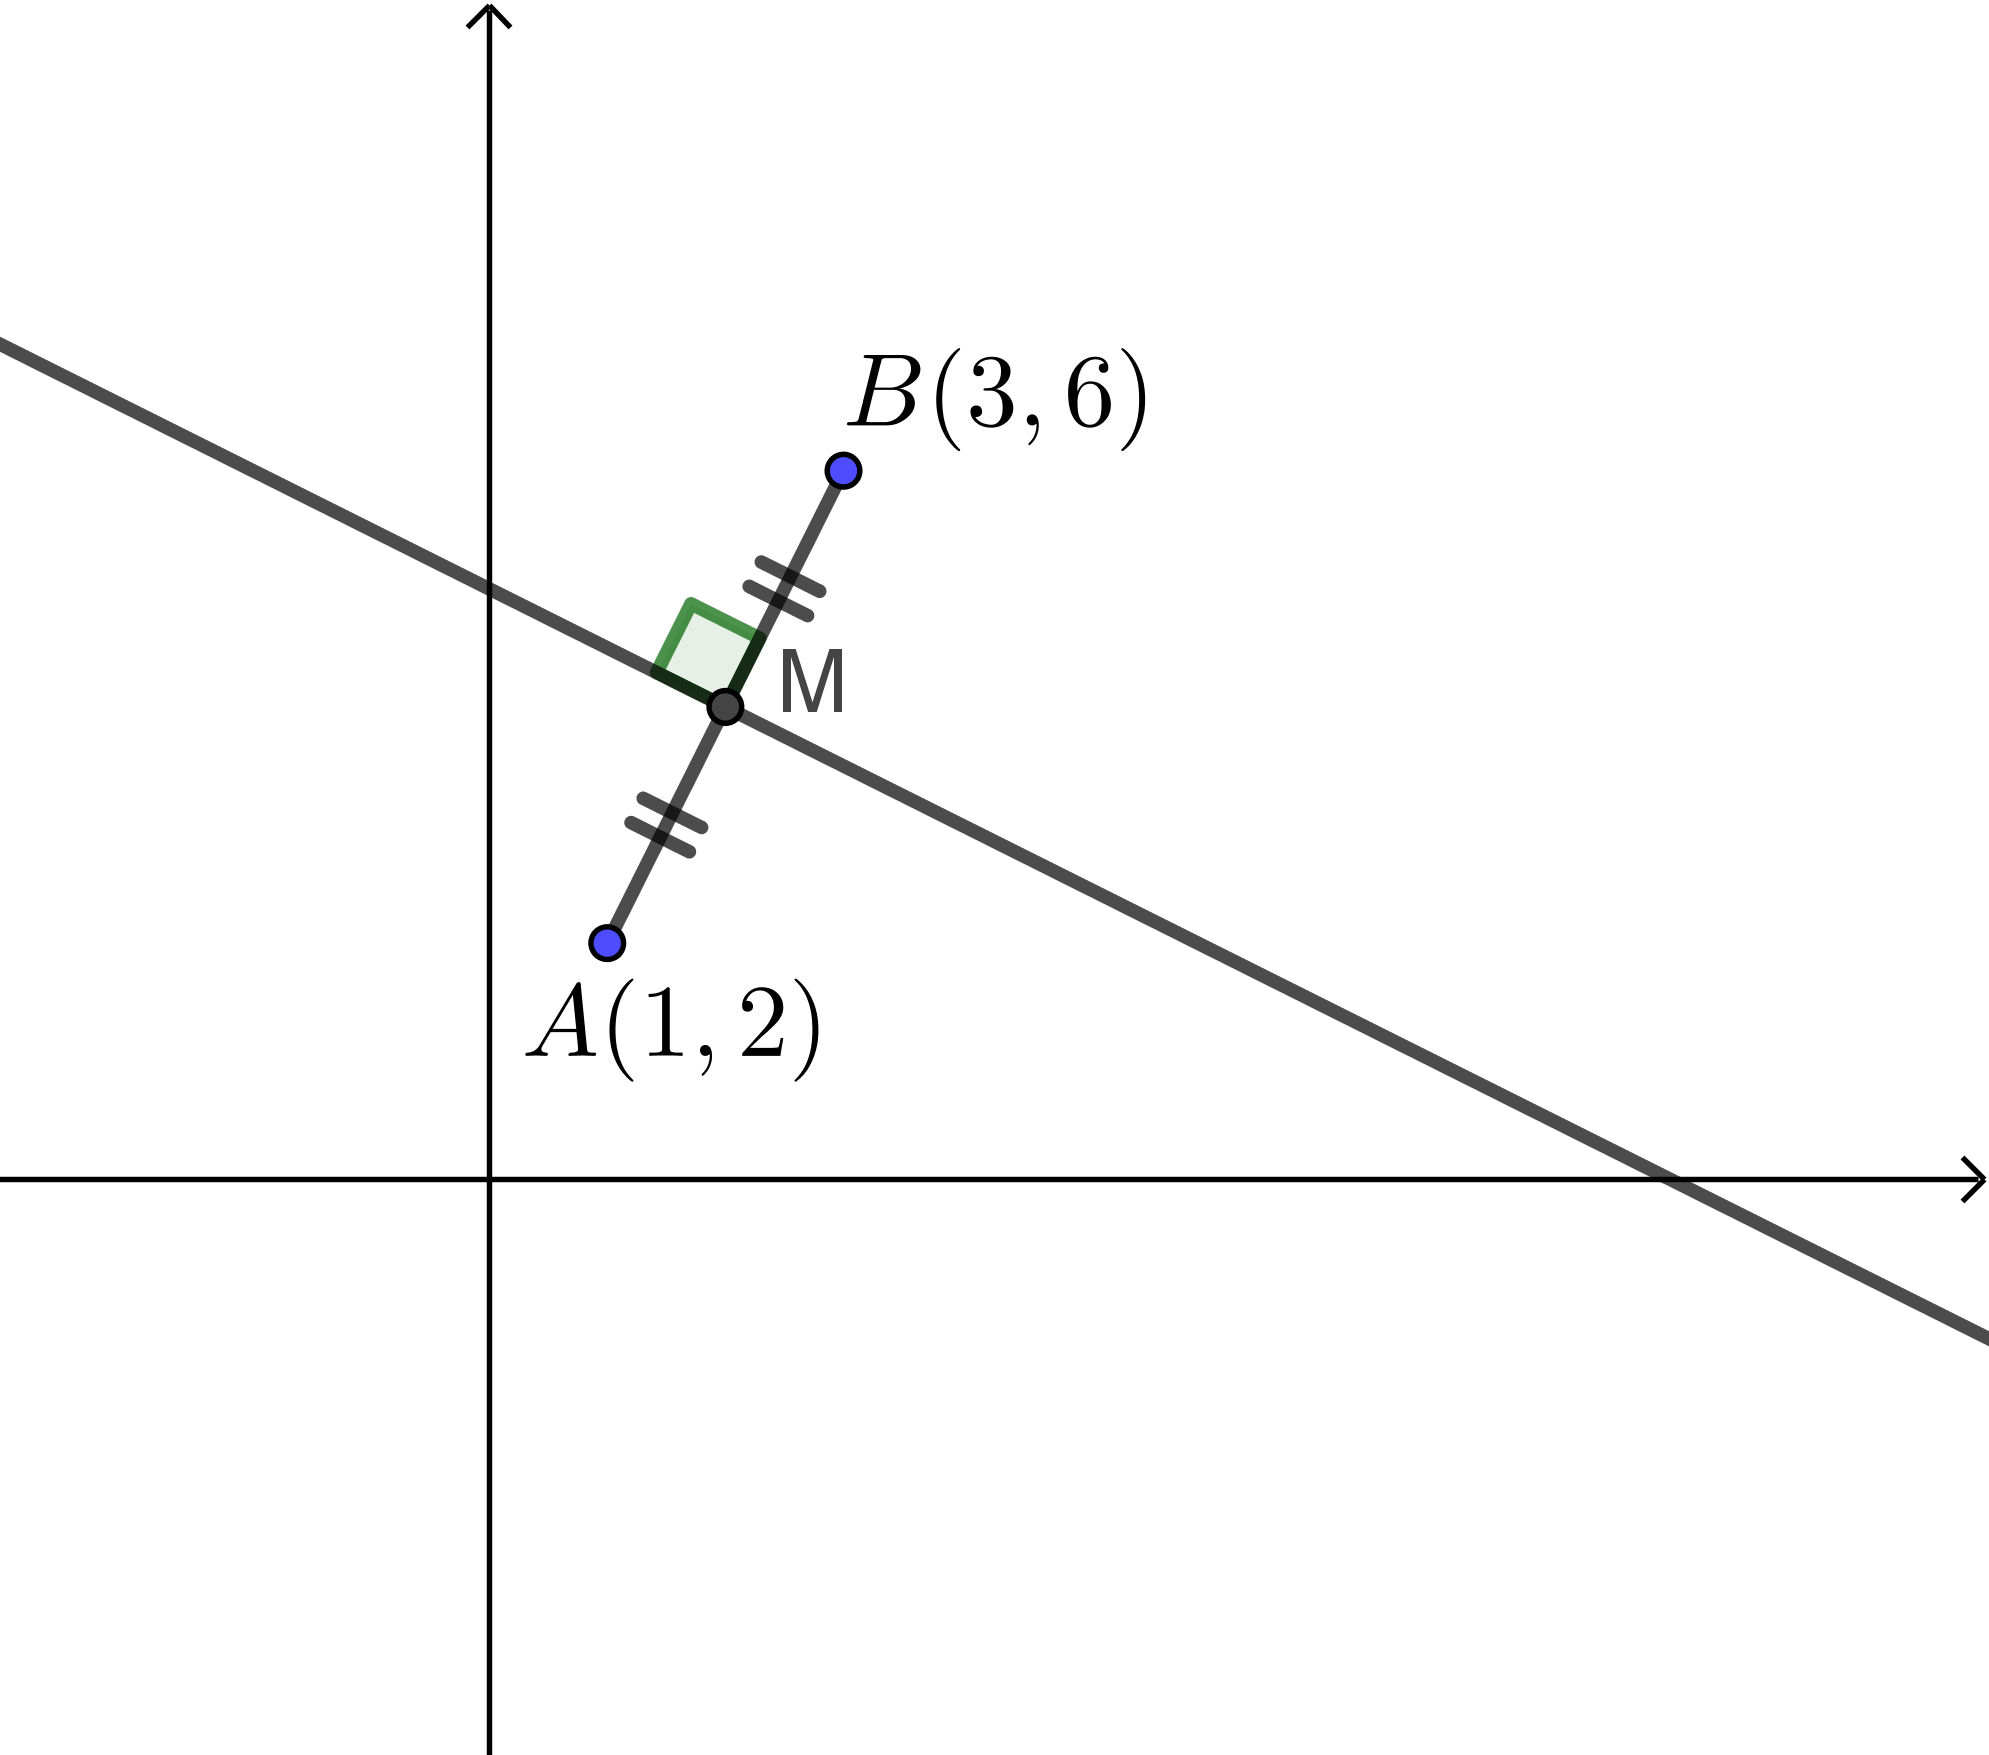
\includegraphics[width=.5\textwidth]{trace_2}
\end{center}
선분 \(AB\)의 기울기는
\[\frac{6-2}{3-1}=2\]
이므로 선분 \(AB\)의 수직이등분선의 기울기는 \(-\frac12\)이다.
또 \(A\)와 \(B\)의 중점
\[M=\left(\frac{1+3}2\:\:,\:\:\frac{2+6}2\right)=(2,4)\]
를 지나므로
\[y=-\frac12(x-2)+4\]
\[y=-\frac12x+5\]
이다.
이것을 더 정리해
\[x+2y-10=0\]
로 쓸 수도 있다.
\end{mdframed}
\par
\begin{mdframed}[frametitle=풀이2]
구하는 점 \(P\)를 \(P=(x,y)\)라고 두고
\(\ov PA=\ov PB\)를 풀면
\begin{gather*}
\sqrt{(x-1)^2+(y-2)^2}=\sqrt{(x-3)^2+(y-6)^2}\\
(x-1)^2+(y-2)^2=(x-3)^2+(y-6)^2\\
4x+8x-40=0\\
x+2y-10=0
\end{gather*}
\end{mdframed}
\ans{선분 \(AB\)의 수직이등분선 \quad또는\quad \(y=-\frac12x+5\) \quad또는\quad \(x+2y-10=0\)}

위의 문제들에서 \textbf{풀이1}의 방법으로 풀 수 있다면 가장 좋지만, 많은 경우에 그렇게 풀리지 않는다. 
그래서 아래와 같은 \textbf{풀이2}의 방법을 사용할 수 있어야 한다.
\begin{mdframed}
%
\theo{자취 문제의 풀이}\label{trace3}
다음과 같은 자취문제
\begin{center}
\fbox{조건 \(A\)를 만족시키는 점 \(P\)의 자취의 방정식을 구하여라.}
\end{center}
를 풀 때에는 다음의 방법으로 푼다.
\begin{enumerate}[label=\roman*)]
\item
\(P=(x,y)\)로 둔다.
\item
주어진 조건 \(A\)를 사용하여 \(x\)와 \(y\) 사이의 관계식을 구한다.
\end{enumerate}
\end{mdframed}

%
\prob{}\label{trace4}
두 점 \(A(-1,2)\), \(B(-1,5)\)에 대해 \(\ov PA=\ov PB\)을 만족시키는 점 \(P\)의 자취의 방정식을 구하여라.
%\procedure{0.3}

%
\prob{}\label{trace5}
두 점 \(A(0,0)\), \(B(3,2)\)에 대해 \(\ov PA=\ov PB\)을 만족시키는 점 \(P\)의 자취의 방정식을 구하여라.
%\procedure{0.3}

\newpage

\prob{}\label{trace6}
점 \(A(4,2)\)에서 직선 \(2x+3y+12=0\) 사이의 거리를 구하여라.

\prob{}\label{trace7}
다음과 같은 \(t\)에 대한 방정식을 풀어라.
\begin{enumerate}
\item
\(|t|=3\)
\item
\(|t-2|=5\)
\item
\(|t+1|=|2t-7|\)
\end{enumerate}

%
\exam{}\label{trace8}
두 직선 \(l:x+7y+3=0\), \(m:x-y-5=0\)에서 같은 거리에 있는 점 \(P\)의 자취의 방정식을 구하여라.

\begin{mdframed}
점 \(P\)를 \(P(x,y)\)로 두면
\begin{gather*}
\frac{|x+7y+3|}{\sqrt{1^2+7^2}}=\frac{|x-y-5|}{\sqrt{1^2+1^2}}\\
%\frac{|x+7y+3|}{5\sqrt2}=\frac{|x-y-5|}{\sqrt2}\\
|x+7y+3|=5|x-y-5|\\
x+7y+3=5(x-y-5)\qquad\text{혹은}\qquad x+7y+3=-5(x-y-5)\\
x-3y-7=0\qquad\text{혹은}\qquad 3x+y-11=0
\end{gather*}
\end{mdframed}
\ans{\(x-3y-7=0\qquad\text{혹은}\qquad 3x+y-11=0\)}
실제로 그림을 그려보면, 답이 되는 두 직선은 \(l\)과 \(m\)의 각이등분선이라는 것을 알 수 있다.
다음 그림에서 \(\triangle PAB\equiv\triangle PAC(RHS)\)이고, 따라서
\[\angle PAB=\angle PAC\]
이기 때문이다.
\begin{center}
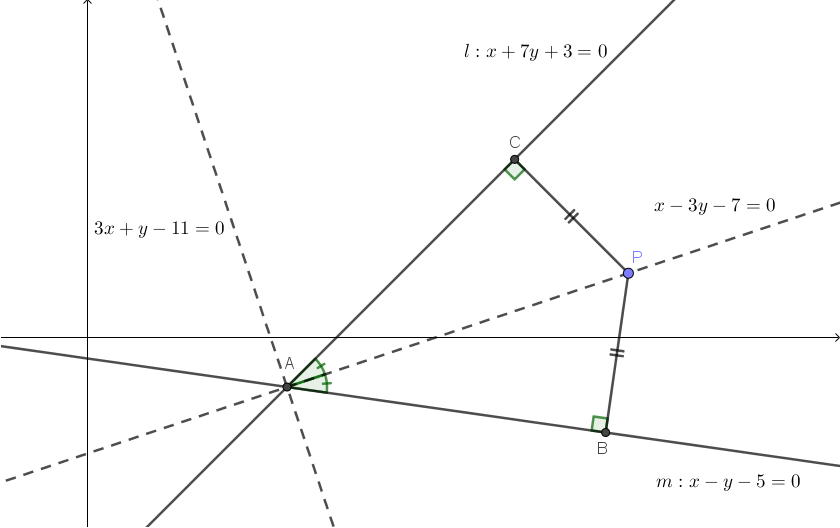
\includegraphics[width=0.8\textwidth]{trace_7}
\end{center}

%
\prob{}\label{trace9}
두 직선 \(l:y=0\), \(m:3x-4y-6=0\)에서 같은 거리에 있는 점 \(P\)의 자취의 방정식을 구하여라.
\procedure{0.15}

%
\prob{}\label{trace10}
두 직선 \(l:2x-y=0\), \(m:x+2y=0\)의 각이등분선들을 구하여라.
\procedure{0.15}

%%c
\section{원의 방정식}

%\begin{mdframed}
%%
%\defi{원}
\emph{원}이란, 
\begin{center}
\fbox{평면 위의 한 점으로부터 일정한 거리에 있는 점들이 이루는 도형}
\end{center}
이다.
%\end{mdframed}

%
\exam{}\label{circle1}
좌표평면 위의 한 점 \(C(3,0)\)으로부터 \(2\)만큼 떨어져 있는 점 \(P\)가 그리는 도형의 방정식을 구하여라.
\begin{mdframed}
\(P=(x,y)\)라고 두자.
\(\ov PC=2\)가 성립해야 하므로
\begin{gather*}
\sqrt{(x-3)^2+(y-0)^2}=2\\
(x-3)^2+y^2=4
\end{gather*}
\end{mdframed}
\ans{\((x-3)^2+y^2=4\)}
다시 말해, 중심이 \(C(3,0)\)이고 반지름의 길이가 \(2\)인 원의 방정식은
\[(x-3)^2+y^2=4\]
이다.
\begin{center}
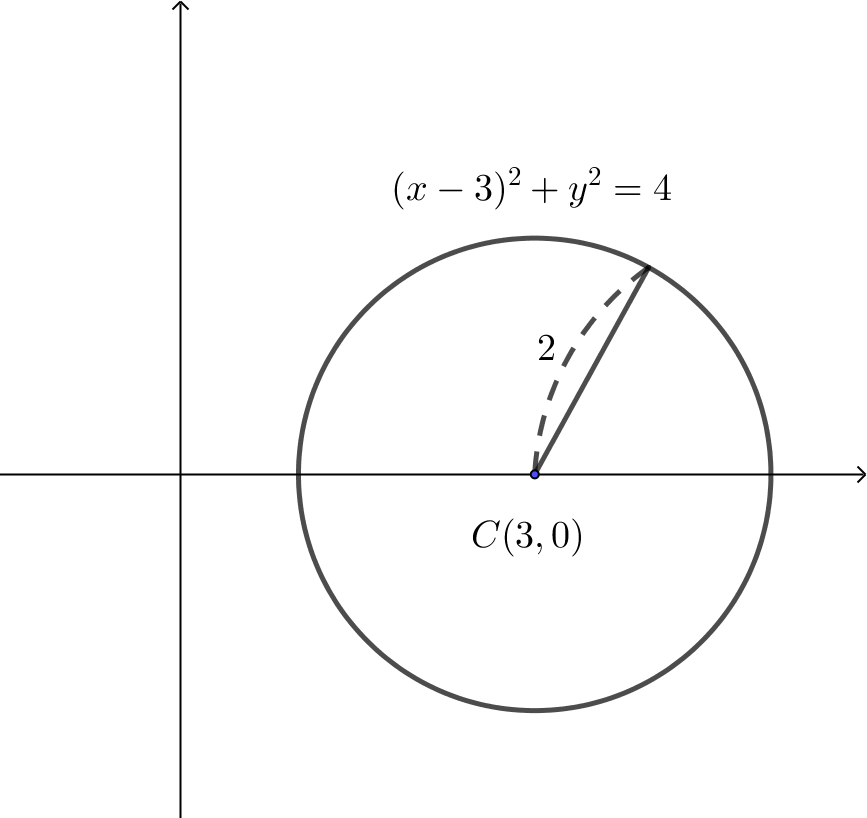
\includegraphics[width=0.6\textwidth]{c_1}
\end{center}

\begin{mdframed}
%
\theo{원의 방정식}\label{circle2}
중심이 \(C(a,b)\)이고 반지름의 길이가 \(r\)인 원의 방정식은
\[(x-a)^2+(y-b)^2=r^2\]
\end{mdframed}
%\proo
%원 위의 한 점을 \(P\)라고 잡고 \(P=(x,y)\)라고 두면, \(\ov PC=r\)로부터
%\begin{gather*}
%\sqrt{(x-a)^2+(y-b)^2}=r\\
%(x-a)^2+(y-b)^2=r^2
%\end{gather*}

%
\prob{다음 원의 방정식을 구하여라.}
\begin{enumerate}\label{circle3}%
\item
중심이 \((2,-3)\)이고 반지름의 길이가 \(4\)인 원 
\item
중심이 원점이고 반지름의 길이가 \(1\)인 원 
\end{enumerate}

%
\exam{}\label{circle4}
원의 방정식 \(x^2-6x+y^2+4y+5=0\)이 나타내는 원의 중심과 반지름의 길이를 구하여라.
\begin{mdframed}
주어진 식을 정리하면
\begin{gather*}
x^2-6x+y^2+4y=-5\\
x^2-6x+9+y^2+4y+4=-5+9+4\\
(x-3)^2+(y+2)^2=8
\end{gather*}
이다.
따라서 원의 중심은 \((3,-2)\)이고, 반지름의 길이는 \(2\sqrt2\)이다.
\end{mdframed}
\ans{\(\text{원의 중심}=(3,-2)\), \(\text{반지름의 길이}=2\sqrt2\)}%\(\text{원의 중심}=(3,-2)\), \

%
\prob{다음 원의 방정식들이 나타내는 원의 중심과 반지름의 길이를 구하여라.}
\begin{enumerate}\label{circle5}%
\item
\(x^2+y^2+4x=0\)
\item
\(2x^2+2y^2-4x+8y+3=0\)
\end{enumerate}

%%circleline
\section{원과 직선의 위치관계}\label{circleline}
\noindent
\begin{minipage}{0.55\textwidth}
%
\exam{}\label{circleline1}
직선 \(y=x+n\)과 원 \(x^2+y^2=4\)의\\
위치관계가 다음과 같을 때, 실수 \(n\)의 값\\
또는 값의 범위를 구하여라.
\begin{enumerate}
\item
만나지 않을 때
\item
한 점에서 만날 때(접할 때)
\item
두 점에서 만날 때
\end{enumerate}
\par\medskip
\end{minipage}
\begin{minipage}{0.4\textwidth}
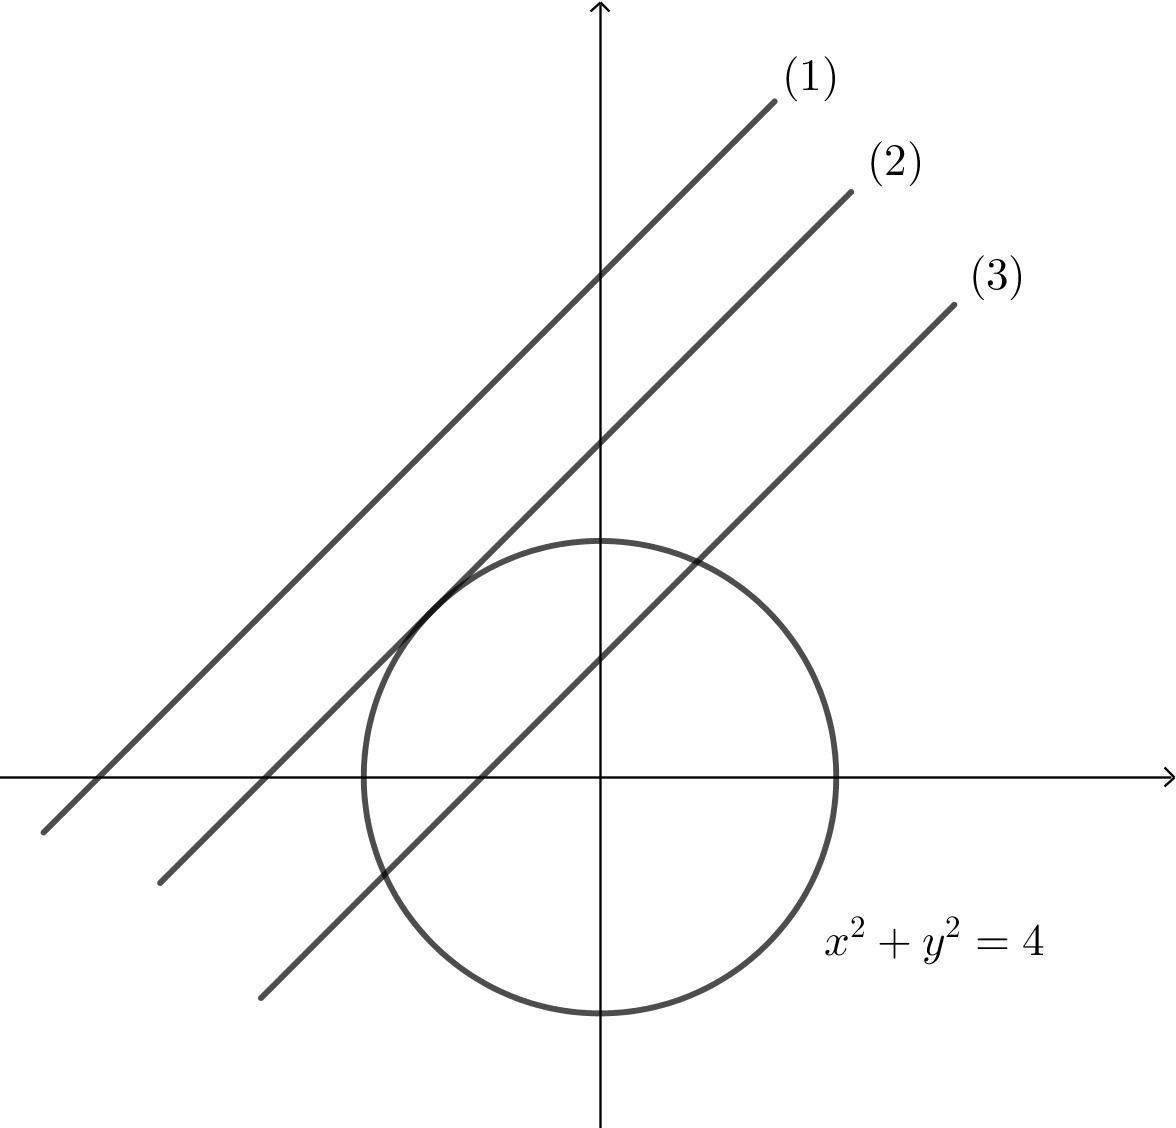
\includegraphics[width=\textwidth]{circleline_1}
\end{minipage}

\begin{mdframed}[frametitle=풀이1,nobreak=false]
(1)이면 교점이 없고, (2)이면 교점이 한 개 있으며, (3)이면 교점이 두 개 있다.
따라서 연립방정식
\[\begin{cases}
y=x+n\\
x^2+y^2=4
\end{cases}\]
의 근의 개수가 (1) \(0\)개, (2) \(1\)개, (3) \(2\)개일 조건을 구하면 된다.
첫 번째 식을 두 번째 식에 대입해 정리하면
\begin{gather*}
x^2+(x+n)^2=4\\
2x^2+2nx+n^2-4=0
\end{gather*}
이다.
\(D/4\)를 계산하면
\[D/4=n^2-2(n^2-4)=-n^2+8\]
이므로
\begin{enumerate}
\item
\(-n^2+8<0\), \(n^2>8\).
따라서
\(n<2\sqrt2\)\:\:혹은\:\:\(n>2\sqrt2\)
\item
\(-n^2+8=0\), \(n^2=8\).
따라서 \(n=\pm2\sqrt2\).
\item
\(-n^2+8>0\), \(n^2<8\).
따라서
\(-2\sqrt2<n<2\sqrt2\).
\end{enumerate}
\end{mdframed}


\begin{mdframed}[frametitle=풀이2]
원점에서부터 직선 \(x-y+n=0\)까지의 거리를 \(d\)라고 하면
\[d=\frac{|0-0+n|}{\sqrt{1^2+(-1)^2}}=\frac{|n|}{\sqrt2}\]
이다.
\par\bigskip
\begin{center}
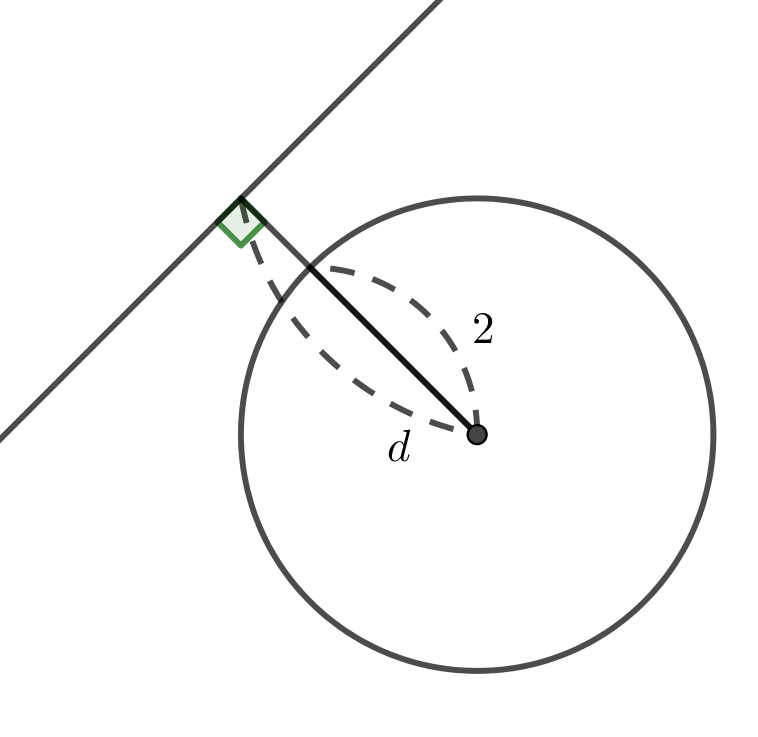
\includegraphics[width=0.25\textwidth]{circleline_1-1}\quad\qquad
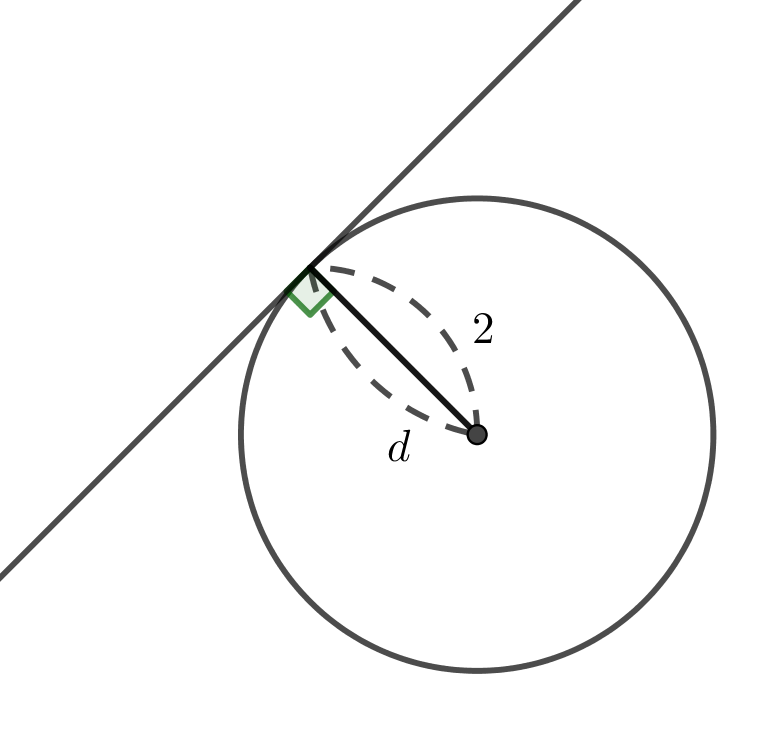
\includegraphics[width=0.25\textwidth]{circleline_1-2}\quad\qquad
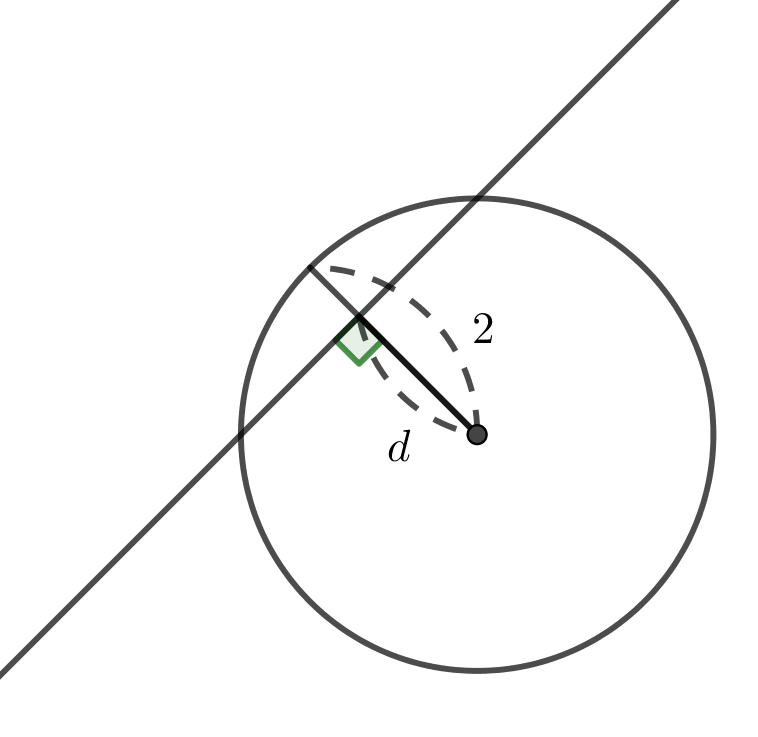
\includegraphics[width=0.25\textwidth]{circleline_1-3}\\
(1) \(d>2\)\qquad\qquad\qquad\quad
(2) \(d=2\)\qquad\qquad\qquad\quad
(3) \(d<2\)
\end{center}
%(1)이면 \(d>r\)이고 (2)이면 \(d=r\)이며 (3)이면 \(d<r\)이다.
\par\bigskip
따라서
\begin{enumerate}\setlength\itemsep{1em}
\item
\(\displaystyle\frac{|n|}{\sqrt2}>2,\quad|n|>2\sqrt2\).\\[1em]
따라서 \(n<2\sqrt2\)\:\:혹은\:\:\(n>2\sqrt2\).
\item
\(\displaystyle\frac{|n|}{\sqrt2}=2,\quad|n|=2\sqrt2\).\\[1em]
따라서 \(n=\pm2\sqrt2\).
\item
\(\displaystyle\frac{|n|}{\sqrt2}<2,\quad|n|<2\sqrt2\).\\[1em]
따라서 \(-2\sqrt2<n<2\sqrt2\).
\end{enumerate}
\end{mdframed}
\ans{
(1) \(n<2\sqrt2\)\:\:혹은\:\:\(n>2\sqrt2\), 
\quad
(2) \(n=\pm2\sqrt2\), 
\quad
(3) \(-2\sqrt2<n<2\sqrt2\)}

\newpage
%
\theo{원과 직선의 위치관계}\label{circleline2}
평면 위에 원과 직선이 있다면 다음의 세 경우 중 하나이다.
\par\bigskip\noindent
\begin{tabu}{X[c]|X[c]|X[c]}
\toprule
만나지 않는다.	&한 점에서 만난다. (접한다.)	&두 점에서 만난다.\\
\hline
 \raisebox{-.5\height}{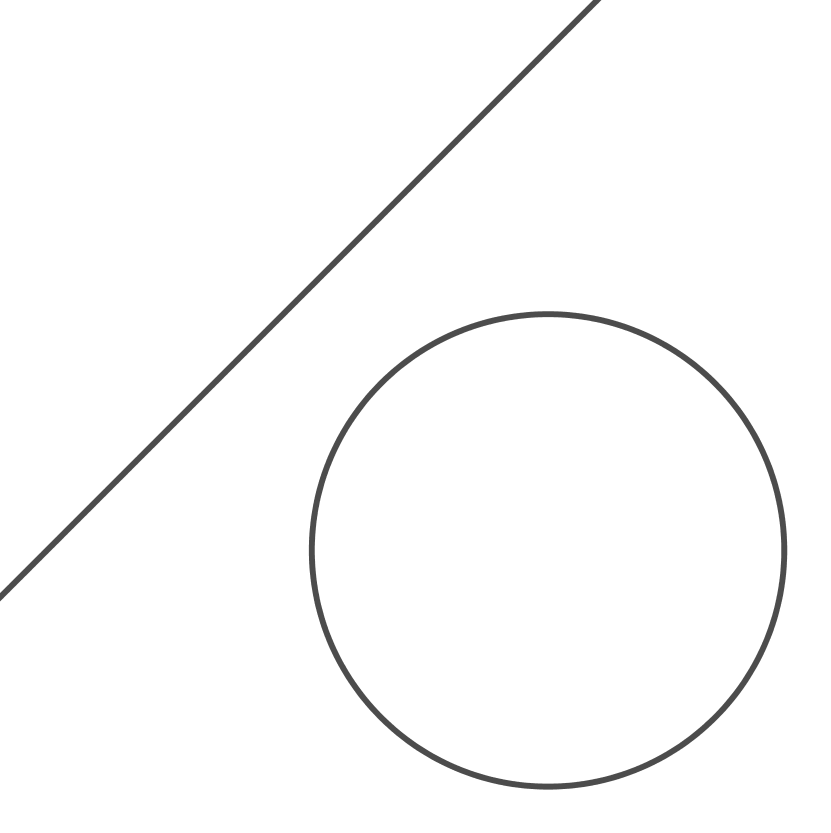
\includegraphics[width=0.24\textwidth]{circleline_0-1}}
&\raisebox{-.5\height}{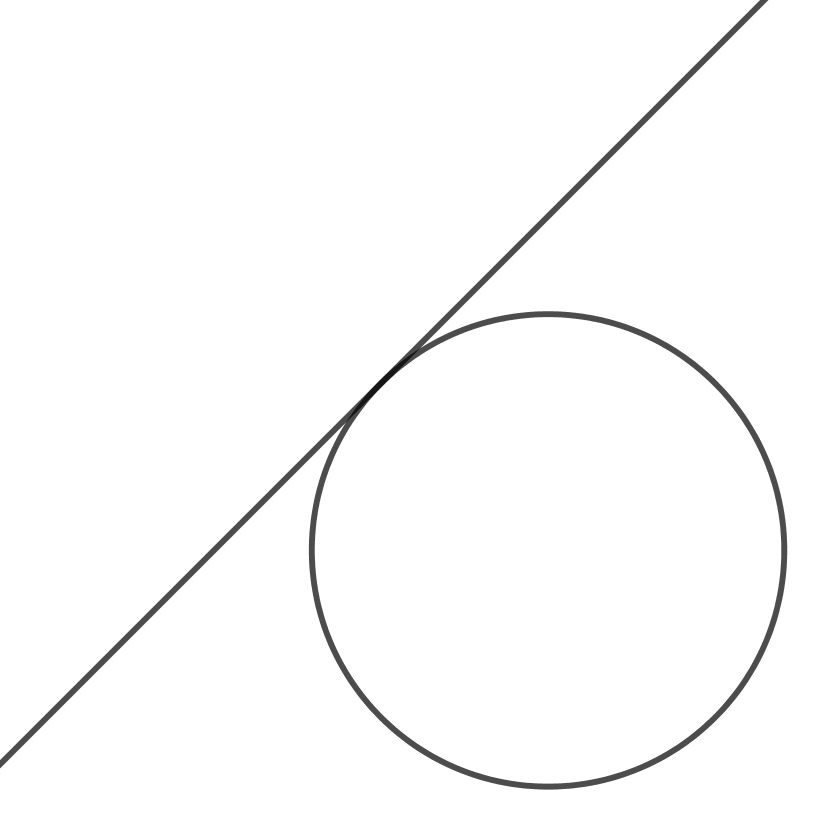
\includegraphics[width=0.24\textwidth]{circleline_0-2}}
&\raisebox{-.5\height}{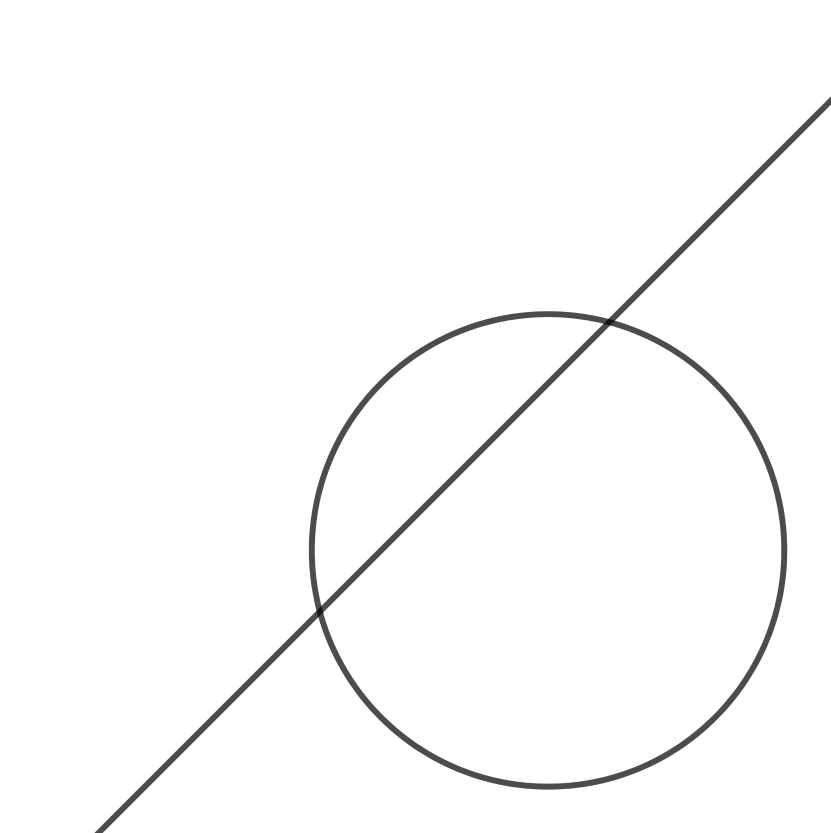
\includegraphics[width=0.24\textwidth]{circleline_0-3}}
\\\hline
\(D<0\)		&\(D=0\)	&\(D>0\)
\\\hline
\(d>r\)		&\(d=r\)	&\(d<r\)
\\\bottomrule
\end{tabu}
\par\bigskip

%
\prob{}\label{circleline3}
직선 \(y=2x+n\)이 원 \((x-1)^2+(y-1)^2=5\)과 두 점에서 만날 때 실수 \(n\)의 값의 범위를 구하여라.
\begin{mdframed}[frametitle=풀이1]
\vspace{.15\textheight}
\end{mdframed}
\begin{mdframed}[frametitle=풀이2]
\vspace{.15\textheight}
\end{mdframed}

%%tangent
\section{원의 접선의 방정식}
%
\exam{}\label{tangent1}
원 \(x^2+y^2=4\) 위의 점 \(A(-1,\sqrt3)\)에서의 접선의 방정식을 구하여라.
\begin{mdframed}
\begin{minipage}{0.6\textwidth}
원의 중심 \(O(0,0)\)와 \(A\)를 이은 선분 \(OA\)의 기울기는
\[\frac{\sqrt3-0}{(-1)-0}=-\sqrt3\]
이므로 접선의 기울기는 \(\frac1{\sqrt3}\)이다.
따라서 접선의 방정식은
\begin{gather*}
y=\frac1{\sqrt3}(x+1)+\sqrt3\\
x-\sqrt3y+4=0
\end{gather*}
\end{minipage}
\:\:
\begin{minipage}{0.35\textwidth}
\begin{center}
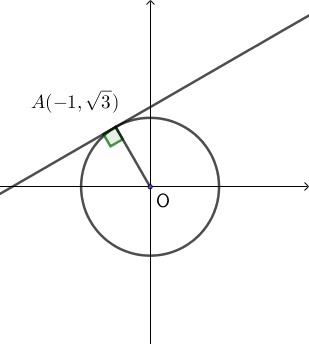
\includegraphics[width=\textwidth]{tangent_1}
\end{center}
\end{minipage}
\end{mdframed}
\ans{\(x-\sqrt3y+4=0\)}

%
\prob{}\label{tangent2}
원 \(x^2+y^2=5\) 위의 점 \(A(2,1)\)에서의 접선의 방정식을 구하여라.

%
\prob{}\label{tangent3}
원 \((x-3)^2+(y-4)^2=25\) 위의 점 \(A(7,7)\)에서의 접선의 방정식을 구하여라.

\newpage
\begin{mdframed}
%
\theo{}\label{tangent4}
원 \(x^2+y^2=r^2\) 위의 점 \(A(x_1,y_1)\)에서의 접선의 방정식은
\[x_1x+y_1y=r^2\]
\end{mdframed}

\bigskip\noindent\textsf{증명\footnotemark)}
\footnotetext{정확한 증명을 위해서는 \(x_1=0\)이거나 \(y_1=0\)인 경우도 고려해야 하지만 생략했다.}
원의 중심 \(O(0,0)\)와 \(A\)를 이은 선분 \(OA\)의 기울기는
\[\frac{y_1-0}{x_1-0}=\frac{y_1}{x_1}\]
이므로 접선의 기울기는 \(-\frac{x_1}{y_1}\)이다.
따라서 접선의 방정식은

\begin{minipage}{0.55\textwidth}
\begin{gather*}
y=-\frac{x_1}{y_1}(x-x_1)+y_1\\
y_1y=-x_1x+{x_1}^2+{y_1}^2\\
y_1y+x_1x={x_1}^2+{y_1}^2
\end{gather*}
\(A(x_1,y_1)\)는 원 위에 있으므로\\
\({x_1}^2+{y_1}^2=r^2\)이다.
이것을 사용하면
\[y_1y+x_1x=r^2\]
를 얻는다.
\qed
\end{minipage}
\begin{minipage}{0.4\textwidth}
\begin{center}
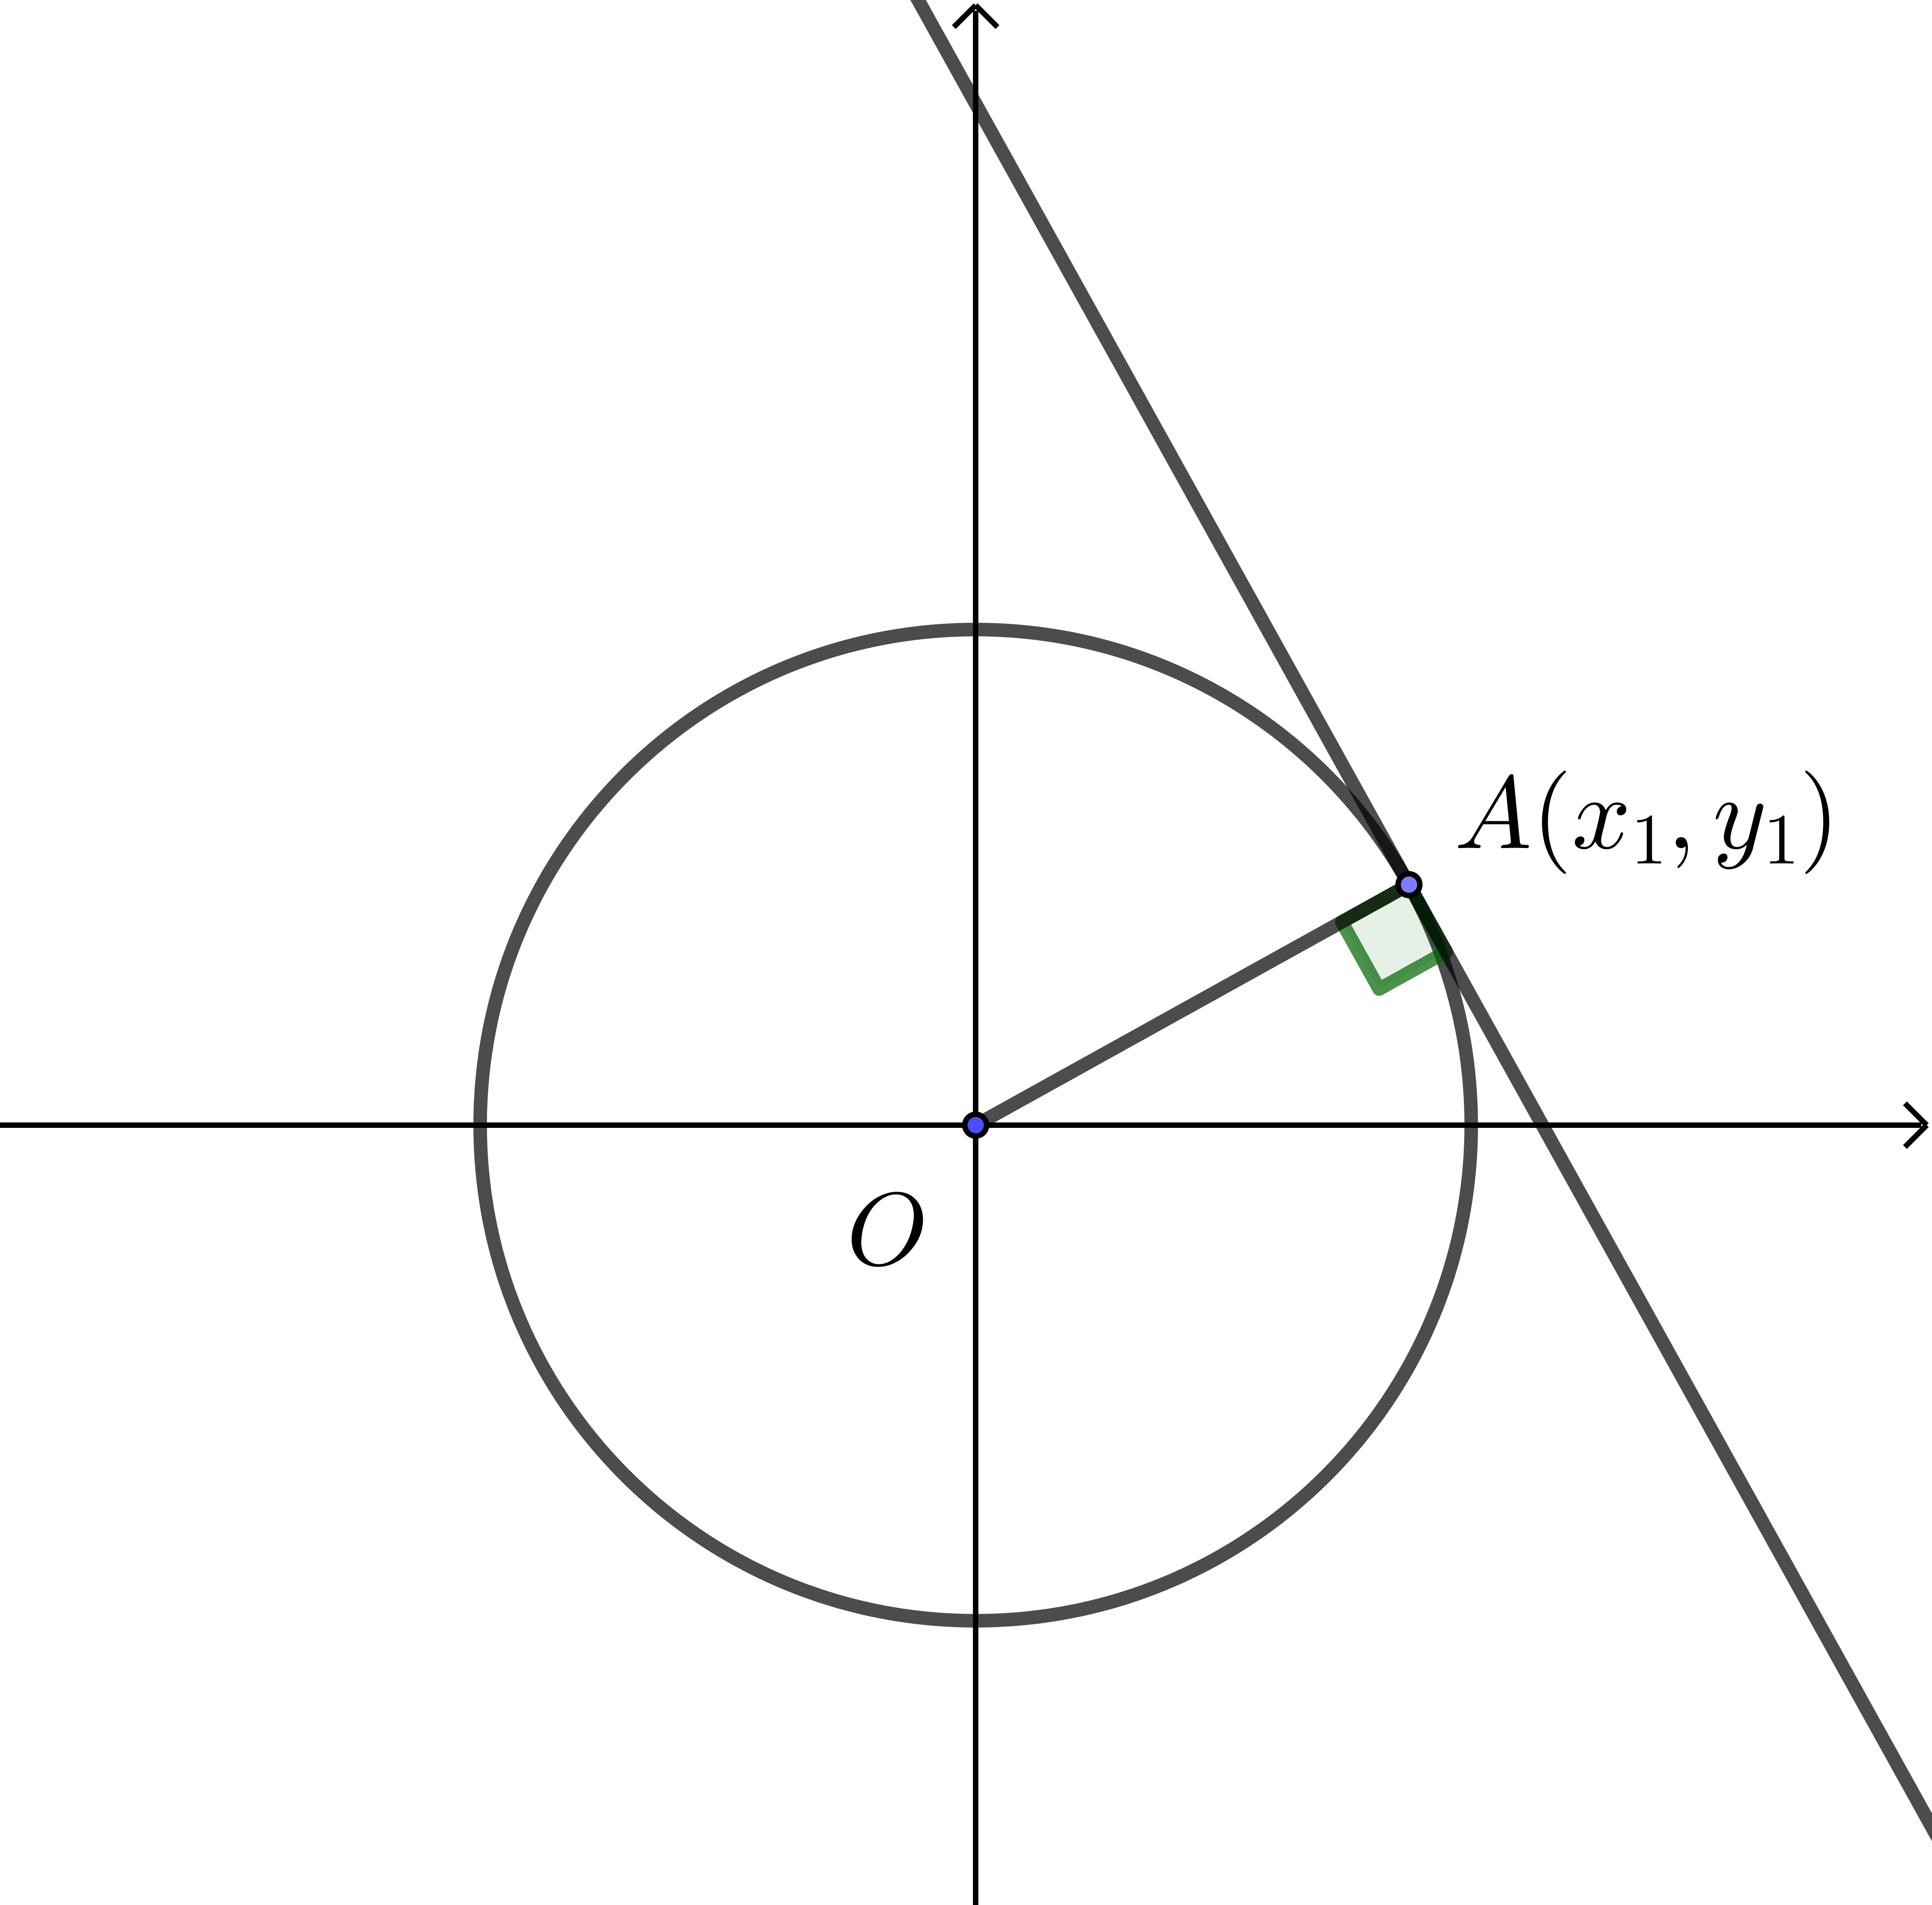
\includegraphics[width=0.9\textwidth]{tangent_4}
\end{center}
\end{minipage}

%
\exam{}\label{tangent5}
예시 \ref{tangent1})\을 정리 \ref{tangent4})의 공식을 적용해 구하면
\[(-1)\cdot x+\sqrt3y=4\]
\[x-\sqrt3y+4=0\]

%
\prob{}\label{tangent6}
문제 \ref{tangent2})\을 정리 \ref{tangent4})의 공식을 적용해 구하여라.

\newpage
%
\exam{}\label{tangent7}
원 \(x^2+y^2=10\)에 접하고 기울기가 \(-3\)인 접선의 방정식을 구하여라.
\begin{mdframed}
접선의 방정식을 \(y=-3x+n\)으로 두고, 예시 \ref{circleline1})에서 사용한 방법을 쓰면 된다.
\bigskip

\noindent\fbox{\textbf{풀이1}}
두 식을 연립하면
\[x^2+(-3x+n)^2=10\]
\[10x^2-6nx+n^2-10=0\]
\[D/4=9n^2-10(n^2-10)=-n^2+100=0\]
\[n=\pm10.\]

\noindent\fbox{\textbf{풀이2}}
원점에서 \(3x+y-n=0\)까지의 거리는
\(\frac{|n|}{\sqrt{10}}\)
이므로
\[\frac{|n|}{\sqrt{10}}=\sqrt{10}\]
에서 \(|n|=10\), \(n=\pm10\).

\noindent\dotfill\hfill

따라서 접선의 방정식은
\[y=-3x\pm10\]
\end{mdframed}

%
\prob{}\label{tangent8}
원 \(x^2+y^2=1\)에 접하고 기울기가 \(-1\)인 접선의 방정식을 구하여라.
\bigskip\bigskip

\newpage
\begin{mdframed}
%
\theo{}\label{tangent9}
원 \(x^2+y^2=r^2\)에 접하고 기울기가 \(m\)인 접선의 방정식은
\[y=mx\pm r\sqrt{1+m^2}\]
\end{mdframed}
\bigskip\noindent\textsf{증명)} 접선의 방정식을 \(y=mx+n\)으로 두자.\bigskip

\noindent\fbox{\textbf{방법1}}
두 식을 연립하면
\begin{gather*}
x^2+(mx+n)^2=r^2\\
(1+m^2)x^2+2mnx+n^2-r^2=0\\
D/4=(mn)^2-(1+m^2)(n^2-r^2)=0\\
-n^2+(1+m^2)r^2=0\\
n=\pm r\sqrt{1+m^2}
\end{gather*}

\noindent\fbox{\textbf{방법2}}
원점에서 \(mx-y+n=0\)까지의 거리는 \(\frac{|n|}{\sqrt{1+m^2}}\)이므로
\[\frac{|n|}{\sqrt{1+m^2}}=r\]
따라서
\[n=\pm r\sqrt{1+m^2}\]
\noindent\dotfill\hfill\\
이 \(n\)값을 \(y=mx+n\)에 대입하면 위의 식이 나온다.

%
\exam{}\label{tangent10}
예시 \ref{tangent7})\을 정리 \ref{tangent9})의 공식을 적용해 구하면
\[y=-3x\pm\sqrt{10}\sqrt{1+(-3)^2}=-3x\pm10\]

%
\prob{}\label{tangent11}
문제 \ref{tangent8})\을 정리 \ref{tangent9})의 공식을 적용해 구하여라.

%%
\section{두 원의 교점을 지나는 도형}
두 직선
\begin{gather*}
l_1:ax+by+c=0\\
l_2:a'x+b'y+c'=0
\end{gather*}
에 대해
\[l_3:(ax+by+c)+m(a'x+b'y+c')=0\]
는 \(l_1\)과 \(l_2\)의 교점을 지나는 직선이었다.

마찬가지로,
두 원
\begin{gather*}
C_1:x^2+y^2+Ax+By+C=0\\
C_2:x^2+y^2+A'x+B'y+C'=0
\end{gather*}
에 대해
\[C_3:(x^2+y^2+Ax+By+C)+m(x^2+y^2+A'x+B'y+C')=0\]
는 \(l_1\)과 \(l_2\)의 교점을 지나는 도형의 방정식이다.
\(C_3\)는 대부분 원을 나타내지만 \(m=-1\)이면 \(x^2\)과 \(y^2\)의 항들이 사라지면서 직선의 방정식이 된다.

\begin{mdframed}
%
\theo{}\label{inter1}
두 원 \(x^2+y^2+Ax+By+C=0\), \(x^2+y^2+A'x+B'y+C'=0\)에 대해
\begin{enumerate}
\item
두 원의 교점을 지나는 원의 방정식은 (\(m\neq-1\))
\[(x^2+y^2+Ax+By+C)+m(x^2+y^2+A'x+B'y+C')=0\]
\item
두 원의 교점을 지나는 직선의 방정식은
\[(x^2+y^2+Ax+By+C)-(x^2+y^2+A'x+B'y+C')=0\]
\end{enumerate}
\end{mdframed}



%%
\section*{답}
\addcontentsline{toc}{chapter}{\protect\numberline{*}답}

\begin{minipage}[t]{.49\textwidth}
%
\an{trace4}
선분 \(AB\)의 수직이등분선 \\또는 \(y=\frac72\)

%
\an{trace5}
선분 \(AB\)의 수직이등분선 \\또는 \(y=-\frac32x+\frac{13}4\) \\또는 \(6x+4y-13=0\)

%
\an{trace6}
\(2\sqrt{13}\)

%
\an{trace7}
\begin{enumerate}
\item
\(t=\pm3\)
\item
\(t=-3,\:\:7\)
\item
\(t=2,\:\:8\)
\end{enumerate}
%\fbox{(3)의 풀이}\\
%\(|A|=|B|\)이면\\
%\(A=B\)이거나 \(A=-B\)이다.
%따라서
%\begin{gather*}
%t+1=2t-7\qquad\text{혹은}\qquad t+1=-(2t-7)\\
%t=8\qquad\text{혹은}\qquad t=2
%\end{gather*}

%
\an{trace9}
\(x-3y-2=0,\:\:3x+y-6=0\)

%
\an{trace10}
\(x-3y=0,\:\:3x+y=0\)

\end{minipage}
\begin{minipage}[t]{.49\textwidth}

%
\an{circle3}
\begin{enumerate}
\item
\((x-2)^2+(y+3)^2=16\)
\item
\(x^2+y^2=1\)
\end{enumerate}

%
\an{circle5}
\begin{enumerate}
\item
\(\text{원의 중심}=(-2,0)\)\\ \(\text{반지름의 길이}=2\)
\item
\(\text{원의 중심}=(1,-2)\)\\ \(\text{반지름의 길이}=\frac{\sqrt{14}}2\)
\end{enumerate}
\end{minipage}

%\begin{minipage}[t]{.49\textwidth}
%
\newpage
%\par\bigskip\noindent\textbf{문제 \ref{circleline3})}\:\:\(-6<n<4\)\par\medskip\noindent
\ann{circleline3}{\(-6<n<4\)}
\fbox{풀이1}
\begin{gather*}
(x-1)^2+(2x+n-1)^2=5\\
x^2-2x+1+4x^2+4(n-1)x+(n-1)^2=5\\
5x^2+2(2n-3)x+n^2-2n-3=0
\end{gather*}
\begin{align*}
D/4
&=(2n-3)^2-5(n^2-2n-3)\\
&=-n^2-2n+24>0
\end{align*}
\begin{gather*}
n^2+2n-24<0\\
(n-4)(n+6)<0\\
-6<n<4
\end{gather*}
\fbox{풀이2}
\begin{gather*}
d=\frac{|2\cdot1+n-1|}{2^2+(-1)^2}=\frac{|n+1|}{\sqrt5}<\sqrt5\\
|n+1|<5\\
-5<n+1<5\\
-6<n<4
\end{gather*}

\begin{minipage}[t]{.49\textwidth}
%
\an{tangent2}
\(2x+y-5=0\)

%
\an{tangent3}
\(4x+3y-49=0\)

%
\an{tangent6}
생략

\end{minipage}
\begin{minipage}[t]{.49\textwidth}
%
\an{tangent8}
\(y=-x\pm\sqrt2\)

%
\an{tangent11}
생략
\end{minipage}

%\end{minipage}
%\begin{minipage}[t]{.49\textwidth}
%\end{minipage}

%%
\section*{요약}
\addcontentsline{toc}{chapter}{\protect\numberline{*}요약}
\begin{enumerate}[label=\arabic*.,itemsep=2em]
\item
자취문제
\begin{enumerate}[label=\roman*)]
\item
\(P=(x,y)\)로 둔다.
\item
주어진 조건 \(A\)를 사용하여 \(x\)와 \(y\) 사이의 관계식을 구한다.
\end{enumerate}
\item
원의 방정식
\[(x-a)^2+(y-b)^2=r^2\]
\item
원과 직선의 위치관계\\[10pt]
\begin{tabu}to0.8\textwidth{X[c]|X[c]|X[c]}
\toprule
만나지 않는다.	&한 점에서 만난다. (접한다.)	&두 점에서 만난다.\\
\hline
 \raisebox{-.5\height}{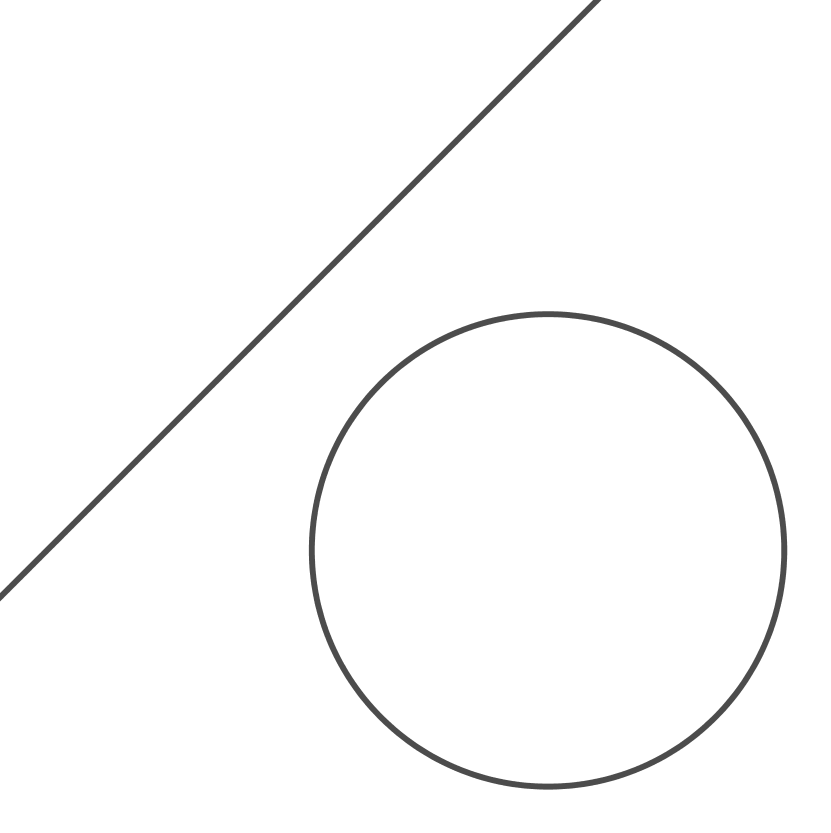
\includegraphics[width=0.24\textwidth]{circleline_0-1}}
&\raisebox{-.5\height}{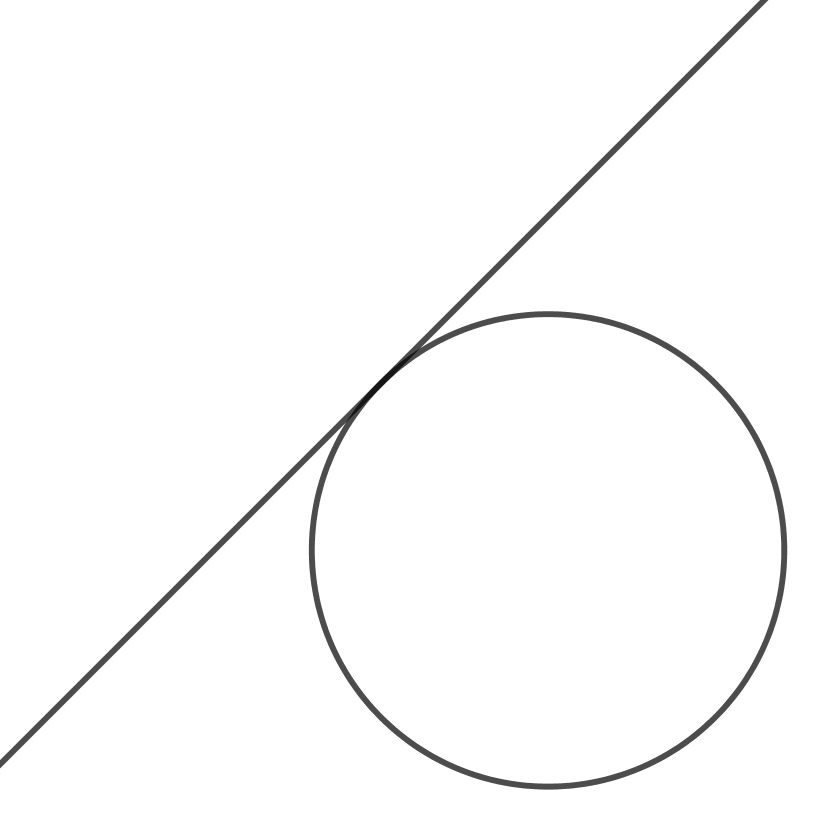
\includegraphics[width=0.24\textwidth]{circleline_0-2}}
&\raisebox{-.5\height}{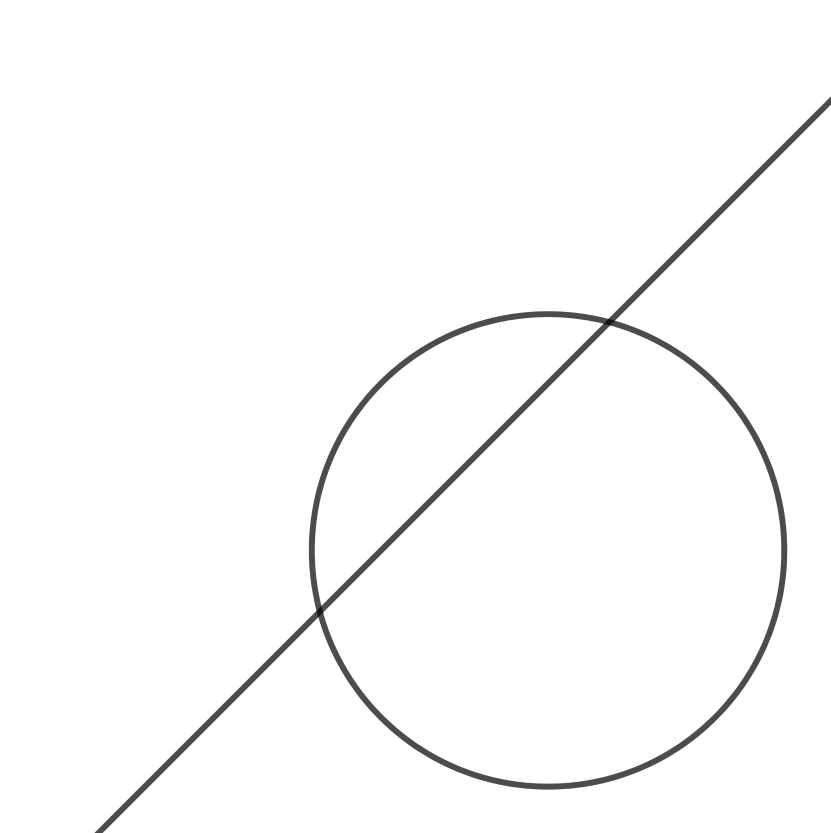
\includegraphics[width=0.24\textwidth]{circleline_0-3}}
\\\hline
\(D<0\)		&\(D=0\)	&\(D>0\)
\\\hline
\(d>r\)		&\(d=r\)	&\(d<r\)
\\\bottomrule
\end{tabu}
\item
원의 접선의 방정식
\begin{itemize}
\item
\(x_1x+y_y=r^2\)
\item
\(y=mx\pm r\sqrt{1+m^2}\)
\end{itemize}
\item
두 원의 교점을 지나는 도형
\[(x^2+y^2+Ax+By+C)+m(x^2+y^2+A'x+B'y+C')=0\]
\end{enumerate}
\end{document}